
\chapter{Preview import}

The preview import window allows
to import a set of previously exported registers
in order to send them in bulk to the modbus slave.
The import window can be opened from the "import" menu, 
via the import button at the bottom or by pressing the
right button on the tables in the main window:

\begin{figure}[H]
\centering
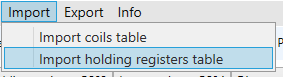
\includegraphics[width=0.35\textwidth]{../Img/Menu_Import.PNG}
\caption{Preview import}
\end{figure}

\begin{figure}[H]
\centering
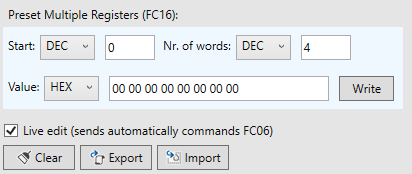
\includegraphics[width=0.35\textwidth]{../Img/PreviewImport_OpenButton.PNG}
\caption{Preview import}
\end{figure}

\begin{figure}[H]
\centering
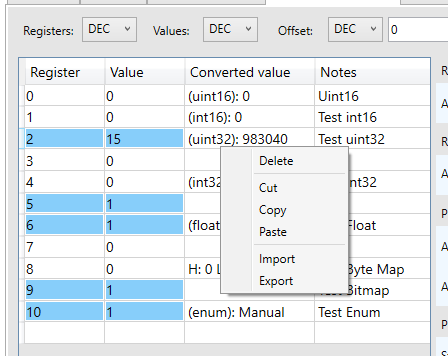
\includegraphics[width=0.50\textwidth]{../Img/PreviewImport_Open.PNG}
\caption{Preview import}
\end{figure}

From the context menu you can either import a set of records
copied from a spreadsheet ("paste") or import a file
.csv/.json ("import"). The "copy" or "cut" commands allow you to copy 
the table displayed on the clipboard and then paste them into a spreadsheet.

\newpage
The preview window appears as follows:

\begin{figure}[H]
\centering
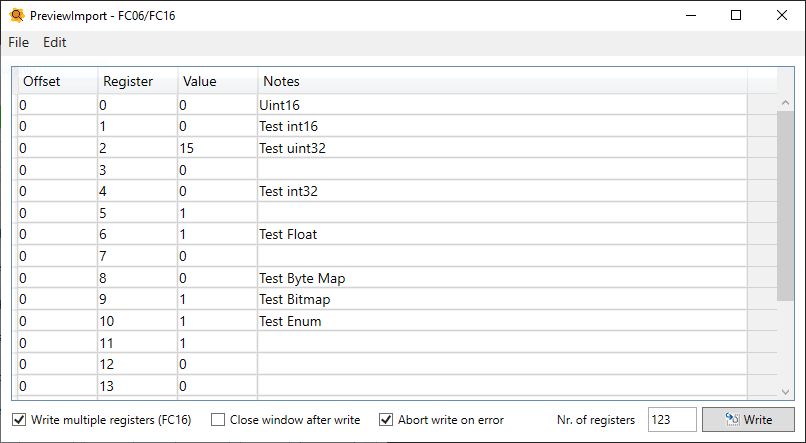
\includegraphics[width=0.85\textwidth]{../Img/PreviewImport_Main.PNG}
\caption{Preview import main window}
\end{figure}

The data displayed in the preview can be copied or pasted
in the window via the context menu:

\begin{figure}[H]
\centering
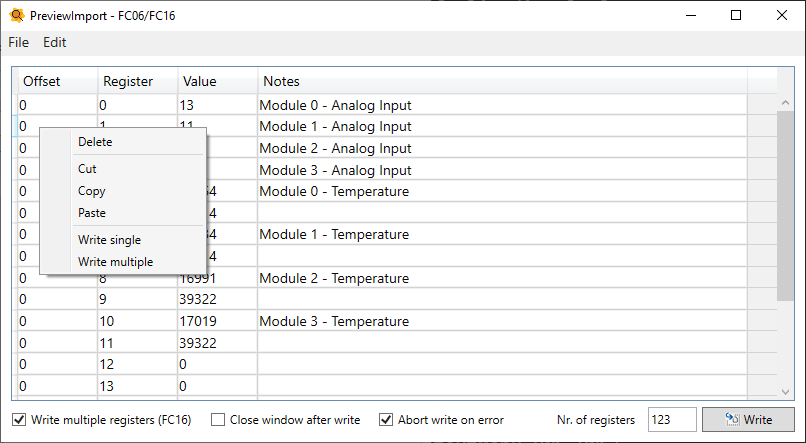
\includegraphics[width=0.85\textwidth]{../Img/PreviewImport_ContextMenu.PNG}
\caption{Preview import context menu}
\end{figure}

The "write single" and "write multiple" commands allow you to send
the displayed registers as a group (FC15/FC16) or individually (FC05/FC06).



